\documentclass{beamer}
\usepackage[MeX]{polski}
\usepackage[utf8]{inputenc}
\usepackage{amsfonts}
\usepackage{graphicx}
\title{Gnidosz błotny}
\author{Dasher}
\date{\today}
\begin{document}
\frame{\titlepage}

\begin{frame}
	\frametitle{Spis Treści}
	\tableofcontents
\end{frame}

\section{Gnidosz błotny}
\begin{frame}{Gnidosz błotny}
(Pedicularis palustris L.) ---  gatunek należący do rodziny zarazowatych. Występuje w Europie, na Kaukazie i w Kanadzie. W Polsce dość częsty na całym niżu.
\begin{figure}
%\section{Kwiat}
\centering
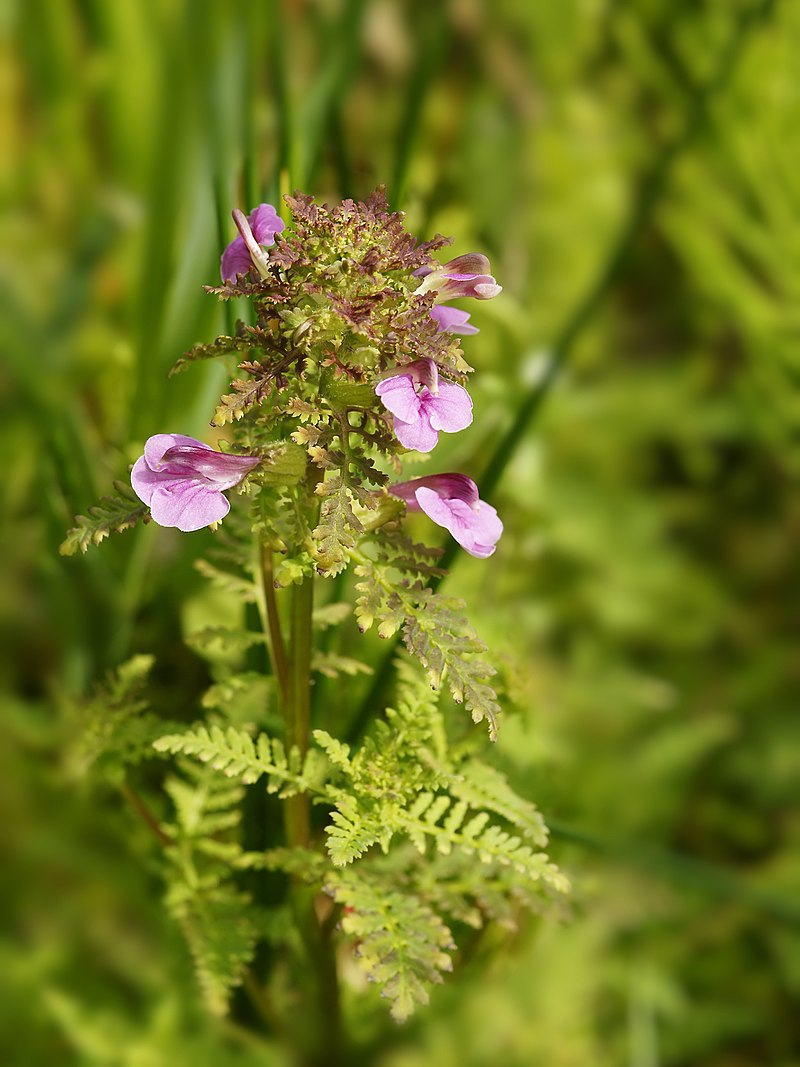
\includegraphics[width=0.25\hsize]{kwiat.jpg}
\caption{Gnidosz błotny}
\end{figure}
\end{frame}

\section{Morfologia}
\subsection{Łodyga}
\begin{frame}{Łodyga}
Wzniesiona, prosta, o wysokości 20-60 cm, górą rozgałęziająca się. Jest prawie naga, w środku pusta.
\end{frame}

\subsection{Liście}
\begin{frame}{Liście}
Pierzastodzielne, o lancetowatych i karbowanych odcinkach, siedzące, żółtozielonego koloru.
\end{frame}

\subsection{Kwiaty}
\begin{frame}{Kwiaty}
Zebrane w luźne grono. Są to kwiaty grzbieciste, wyrastają w kątach liści na krótkich szypułkach. Mają dwuwargowy rozdęty kielich z pierzastowciętymi i odgiętymi do tyłu łatkami. Jest to kielich trwały, pozostający po przekwitnięciu. Purpurowa lub różowa korona o rurce dłuższej od kielicha, orzęsiona na bokach. Dolna warga zamyka wejście do gardzieli korony, górna, dwuząbkowa warga jest ściśnięta po bokach. 1 słupek, 4 dwusilne pręciki ukryte pod górną wargą. Miodniki umieszczone u podstawy słupka, ale dostęp do nich utrudniają włoski pręcików.
\end{frame}

\subsection{Owoc}
\begin{frame}{Owoc}
Dwukomorowa, otoczona kielichem, okrągła torebka.
\end{frame}

\subsection{Korzeń}
\begin{frame}{Korzeń}
Posiada ssawki, którymi wrasta w korzenie sąsiadujących roślin.
\end{frame}

\section{Biologia i ekologia}
\begin{frame}{Biologia i ekologia}
Roślina jednoroczna lub dwuletnia, hemikryptofit. Jest półpasożytem. Na użytkowanych łąkach uznawana za chwast, gdyż osłabia sąsiednie rośliny wysysając z nich wodę i sole mineralne. Roślina miododajna, owadopylna, kwitnie od maja do lipca. Zapylana jest przeważnie przez trzmiele. Roślina trująca.

Rośnie na mokrych łąkach i torfowiskach. W górach występuje po regiel dolny. W klasyfikacji zbiorowisk roślinnych gatunek charakterystyczny dla klasy (Cl.) Scheuchzerio-Caricetea nigrae.
\end{frame}

\section{Zmienność}
\begin{frame}{Zmienność}
Występuje w 2 podgatunkach:
\begin{itemize}
\item Pedicularis palustris L. subsp. opsiantha (Ekman) Almquist z Uznamu --- o koronie średnicy ok. 15 mm i rozgałęzieniach łodygi o grubości prawie równej ich długości.

\item Pedicularis palustris L. subsp. palustris.
\end{itemize}
\end{frame}

\section{Zagrożenia i ochrona}
\begin{frame}
W latach 2004-2014 roślina była objęta w Polsce ścisłą ochroną gatunkową, od 2014 roku podlega ochronie częściowej. Roślina została umieszczona w Polskiej Czerwonej Księgi Roślin jako gatunek narażony na wymarcie (kategoria zagrożenia VU). Tę samą kategorię zagrożenia otrzymała w Czerwonej liście roślin i grzybów Polski (2006, 2016). Zagrożeniem jest zanikanie stanowisk wynikające z osuszania terenów podmokłych i przekształcania ich w łąki i inne tereny użytkowe. Wiele stanowisk znajduje się na obszarach chronionych, m.in. w Białowieskim, Wielkopolskim i Tatrzańskim Parku Narodowym.
\end{frame}

\end{document}